Se emplearon dos fuentes de voltaje y una fuente de corriente para llevar a cabo
el experimento.
Una de las fuentes de voltaje se conectó a un voltímetro y al cañón de
electrones, proporcionando el potencial de aceleración.
La segunda fuente se conectó a otro voltímetro y al capacitor encargado de
generar la deflexión, actuando como el potencial de deflexión.
La fuente de corriente se conectó a un amperímetro y a las bobinas de Helmholtz,
permitiendo determinar el campo magnético inducido.
El esquema del montaje experimental se muestra en la \cref{fig:set-up}.

\begin{figure}[htbp!]
  \centering
  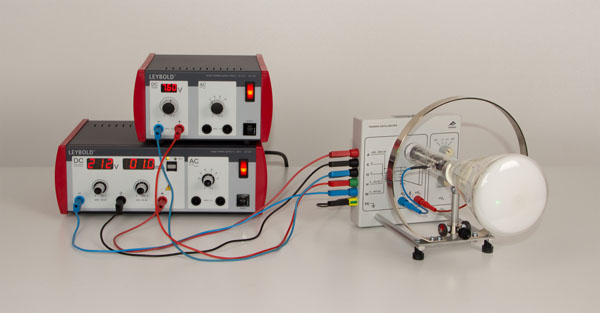
\includegraphics[width=0.8\linewidth]{./images/braun-tube.jpg}
  \caption{Montaje experimental.}
  \label{fig:set-up}
\end{figure}

Además, en una hoja milimetrada se marcó un punto de referencia, a partir del
cual se trazaron tres marcas adicionales a diferentes distancias.
Las posiciones relativas de estas marcas son las distancias entre el punto de 
referencia y cada una de las marcas de --- cm, --- cm y --- cm, respectivamente.
%TODO: Add distances between points

Se suministró una diferencia de potencial al cañón de electrones, generando un
haz de electrones que impactó en el extremo opuesto del tubo de vidrio cubierto
con un material fluorescente, lo que permitió observar un punto de luz.
Sobre este punto se posicionó la hoja milimetrada, de modo que el punto de
referencia coincidiera con el punto de luz y las otras tres marcas quedaran
alineadas debajo del mismo.

Posteriormente, se aplicó un potencial al capacitor, provocando la deflexión del
haz de electrones.
El valor del potencial se ajustó hasta que el punto de luz coincidiera con una
de las marcas en la hoja milimetrada, registrándose tanto la distancia como el
potencial aplicado.
A continuación, se suministró corriente a las bobinas de Helmholtz, ajustándose
para que el punto de luz deflectado volviera a su posición original, es decir,
al punto de referencia.
Este procedimiento se repitió para las tres marcas, y los valores de potencial
de aceleración utilizados fueron de --- V.
%TODO Añadir los valores de potenciales
